\documentclass[conference]{IEEEtran}
\IEEEoverridecommandlockouts

\usepackage{cite}
\usepackage{amsmath,amssymb,amsfonts}
\usepackage{algorithmic}
\usepackage{graphicx}
\usepackage{textcomp}
\usepackage{xcolor}
\usepackage{booktabs}
\usepackage{multirow}
\usepackage[hidelinks]{hyperref}
\usepackage{float}
\usepackage{array}
\usepackage[compatibility=false]{caption}
\captionsetup[figure]{font=footnotesize}
\captionsetup[table]{font=footnotesize}
\usepackage{subcaption}
\usepackage{url}

\graphicspath{{./}{./Report/}}

\def\BibTeX{{\rm B\kern-.05em{\sc i\kern-.025em b}\kern-.08em
    T\kern-.1667em\lower.7ex\hbox{E}\kern-.125emX}}

\begin{document}

\title{From Skeleton to Score: A Feature-Engineered Pipeline for Automated Exercise Form Grading\\
}

\author{
\IEEEauthorblockN{Shashank Dimri}
\IEEEauthorblockA{
\textit{School of Computer Science, AI Cluster} \\
\textit{University of Petroleum and Energy Studies}\\
Dehradun, Uttarakhand, India \\
Shashank.124397@stu.upes.ac.in \\
Shashanklucky190@gmail.com \\
ORCID: 0009-0007-5064-5834}
\and
\IEEEauthorblockN{Dr.\ Swati Rastogi}
\IEEEauthorblockA{
\textit{School of Computer Science, AI Cluster} \\
\textit{University of Petroleum and Energy Studies}\\
Dehradun, Uttarakhand, India \\
ORCID: 0000-0002-2084-2956}
}

\maketitle

\begin{abstract}
Grading push-ups, sit-ups, and pull-ups by eye is how most military recruitment boards and school fitness programmes still work. An evaluator watches, counts reps, and decides whether each one looked right. The process is slow and the outcomes vary from one evaluator to the next.

We built a web platform that does this automatically. A smartphone camera records the exercise; Google MediaPipe pulls out 33 skeletal landmarks per frame; and we compute 28 numbers from the landmark sequence --- things like how far the elbow bends, whether the torso stays rigid, how symmetric the left and right sides are, and how consistent the pacing is. A Random Forest classifier trained on labelled videos then decides ``correct'' or ``foul,'' while a simple linear model fixes the systematic miscounts of our heuristic rep counter. Everything runs through a React frontend, a Flask API, MongoDB, and Google Drive. On 79 labelled videos across three exercises, stratified five-fold cross-validation gives 91.3\% accuracy and 90.5\% F1. The rep calibrator cuts counting error from 2.1 reps to 0.4 --- better than we initially expected from such a simple correction model. The features the classifier relies on most are the ones any coach would point to first: range of motion, depth, and torso alignment.
\end{abstract}

\begin{IEEEkeywords}
pose estimation, exercise form classification, repetition counting, random forest, biomechanical features, physical fitness testing, MediaPipe, sports technology
\end{IEEEkeywords}

%=====================================================================
\section{Introduction}
%=====================================================================

Every year, the Sports Authority of India (SAI) runs fitness camps at about 50 centres across the country, testing candidates on push-ups, sit-ups, pull-ups, and a handful of other exercises~\cite{sai2023}\footnote{SAI's testing protocols are publicly documented at \url{https://sai.gov.in}, though the specific form criteria used by evaluators during field assessments are not formally codified --- a gap that partly motivated this work.}. The setup has not changed much in decades. A trained evaluator watches each person, counts reps on their fingers, and makes a call --- correct or foul --- for every repetition. It works, but not well enough.

The problems are well known. Atkinson and Nevill~\cite{atkinson1998} showed that inter-rater reliability in field-based fitness testing rarely gets above 80\%, and Hopkins~\cite{hopkins2000} confirmed this in a broader meta-analysis a couple of years later. Beyond inconsistency, there is a throughput bottleneck: one evaluator can handle maybe 12--15 candidates per hour. And then there is geography. India has over 740 districts, but SAI centres sit in only about 50 cities. A promising 16-year-old in rural Odisha has to spend money and miss school just to get tested.

Computer vision offers a way out. OpenPose~\cite{cao2017} showed in 2017 that Part Affinity Fields could track multiple people's joints in real time. Since then, Google released MediaPipe~\cite{bazarevsky2020,lugaresi2019}, which gets 33~body keypoints on a phone CPU without needing a GPU at all. Kim \textit{et al.}~\cite{kim2023} benchmarked it against optical motion capture and found sub-centimetre error for upper-body landmarks under decent lighting. So the raw pose data is there.

But knowing where someone's elbow is does not tell you whether their push-up was any good. That requires measuring how far the elbow actually bends, whether the hips sag, whether the left side matches the right, and whether the athlete keeps a steady rhythm. Fig.~\ref{fig:skeleton_compare} shows the difference at a glance --- the correct form on the left maintains a straight body line (176\textdegree) with arms tucked close, while the foul form on the right has flared elbows and a collapsed torso alignment (113\textdegree). Existing research has tackled pieces of this puzzle --- repetition counting~\cite{dwibedi2020}, diving quality scores~\cite{parmar2019}, skeleton-based action recognition~\cite{simonyan2014} --- but nobody, as far as we can tell, has built the whole thing: a system where an administrator uploads labelled videos, a model trains on them, new submissions get graded, a human can review and override, and the model retrains on the corrections. That is what we did.

\begin{figure}[ht]
    \centering
    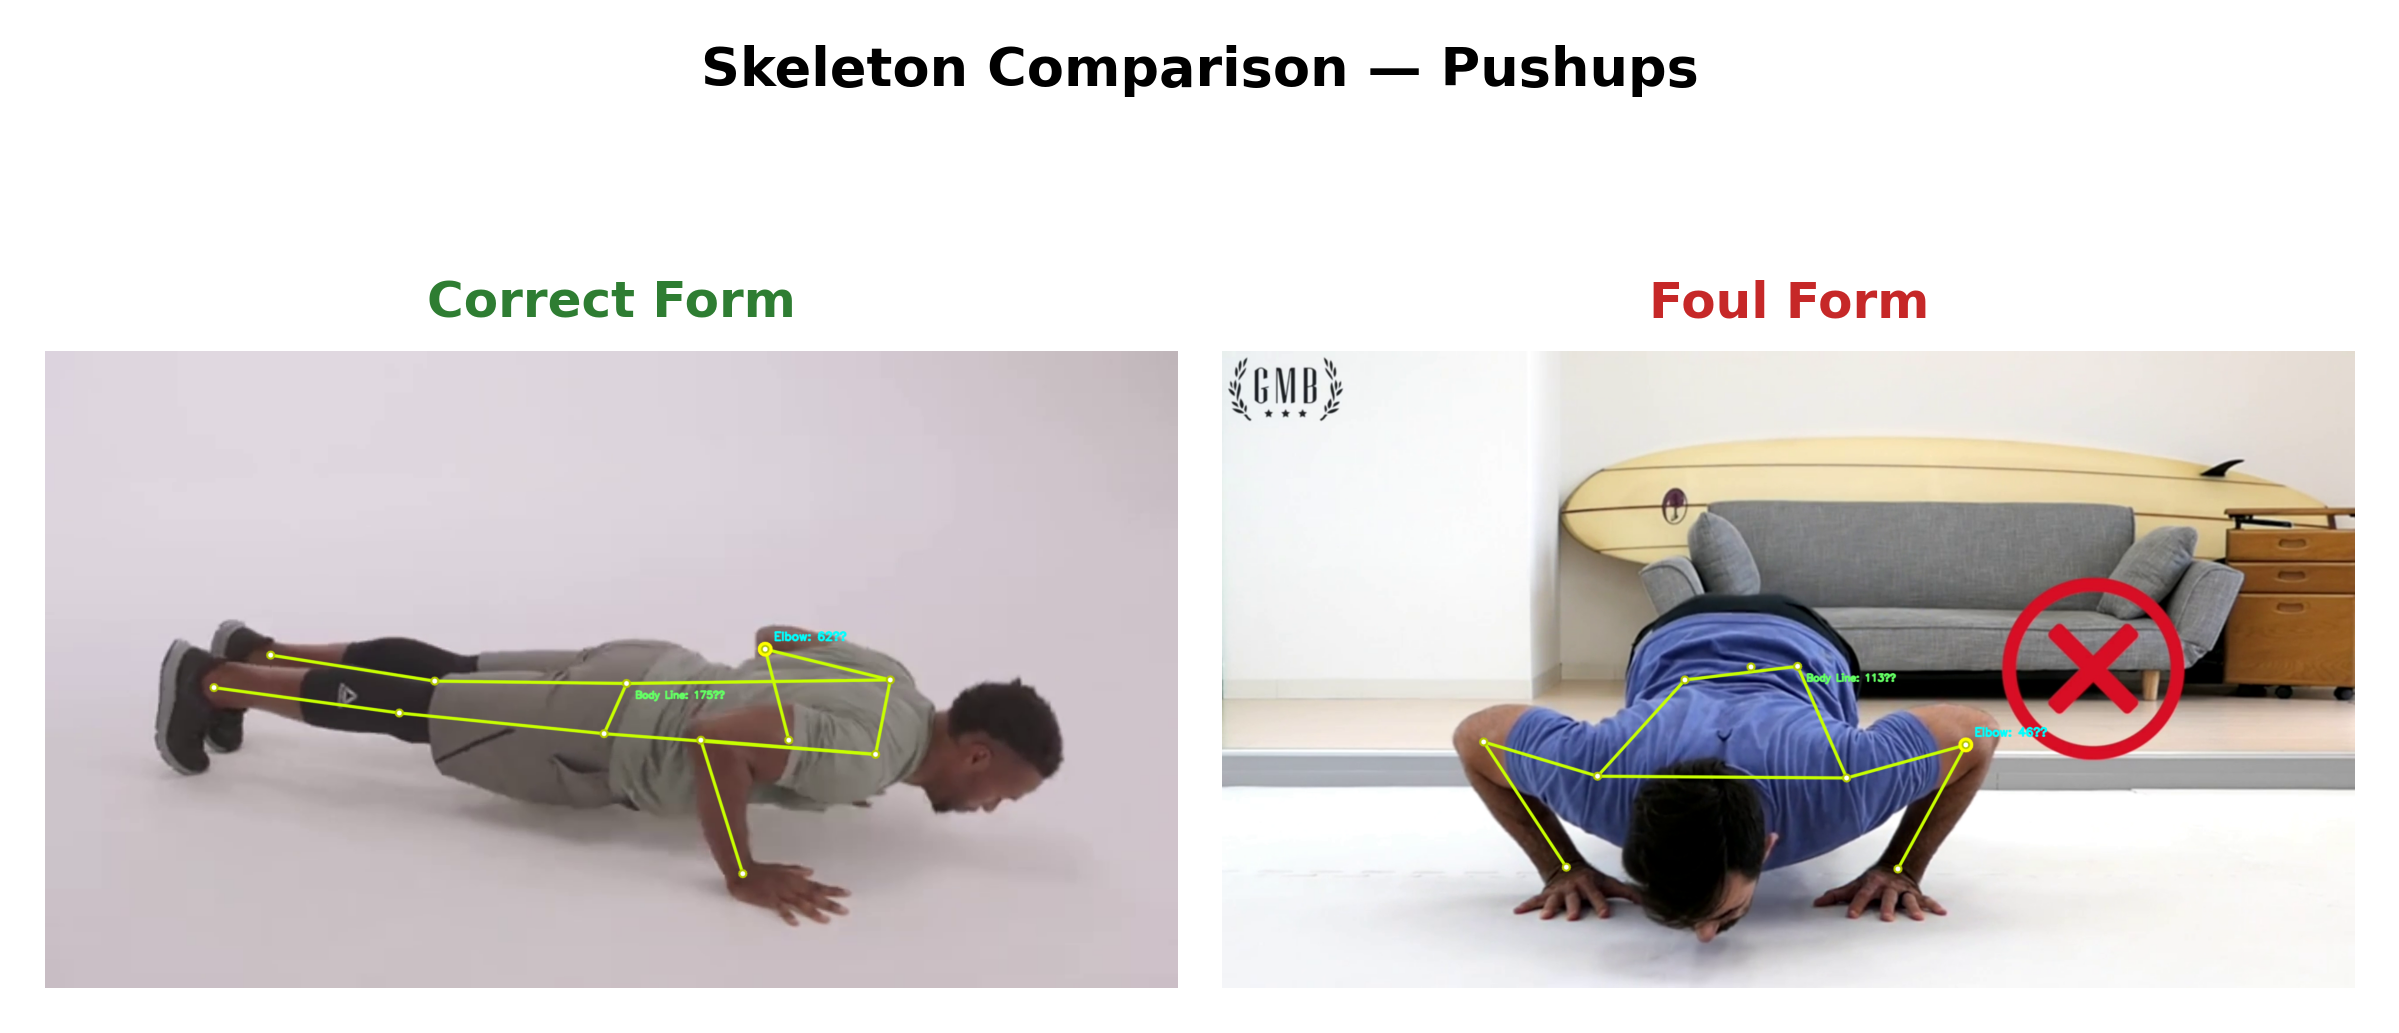
\includegraphics[width=\columnwidth]{skeleton_correct_vs_foul.png}
    \caption{Skeleton overlay comparison for push-ups. Left: correct form --- arms tucked close to the body, straight back with a body-line angle of 176\textdegree. Right: foul form --- flared elbows, collapsed torso alignment (body-line angle drops to 113\textdegree). Joint angles are annotated at the elbow and hip.}
    \label{fig:skeleton_compare}
\end{figure}

The work reported here has four parts. We engineered a compact feature vector --- 28 biomechanical descriptors in total --- from skeletal pose sequences, covering everything from joint angle ranges to rep-to-rep timing consistency. Those features feed a two-stage pipeline: a Random Forest that classifies form as correct or foul, paired with a linear regressor that patches the systematic bias in our heuristic rep counter. Both models are trained per exercise type. We wrapped the whole thing in a web application where athletes submit videos, administrators review and label them, and updated models can be retrained with a single button click. Finally, we evaluate the system with proper rigour --- stratified cross-validation, an ablation study pulling out feature groups one at a time, and head-to-head comparison against logistic regression and SVM baselines --- rather than reporting a single accuracy number and calling it a day.

%=====================================================================
\section{Related Work}
%=====================================================================

\subsection{Pose Estimation}
The pose estimation landscape changed in 2017 when Cao \textit{et al.}~\cite{cao2017} showed that Part Affinity Fields could handle multiple people at once without first running a person detector. That was important for crowded scenes but overkill for our use case --- one person exercising in front of a camera. Bazarevsky \textit{et al.}~\cite{bazarevsky2020} went in the other direction with BlazePose, optimising for a single person on mobile hardware. MediaPipe~\cite{lugaresi2019} packaged this into a drop-in framework. We use it at model complexity 1, which is the sweet spot between speed and accuracy on a laptop webcam.

Dill \textit{et al.}~\cite{dill2023} ran a careful accuracy study specifically for exercise scenarios and found that MediaPipe holds up well when the camera angle is reasonable and body visibility stays above 50\%, but accuracy falls off quickly when the subject turns sideways or the room gets dark. We saw the same pattern in our data and ended up adding visibility-based features to help the classifier account for it.

\subsection{Repetition Counting}
Dwibedi \textit{et al.}~\cite{dwibedi2020} trained RepNet to count repetitions by spotting temporal self-similarity in video embeddings. Hu \textit{et al.}~\cite{hu2022} pushed this further with TransRAC, using a transformer to capture multi-scale correlations. Both get impressive results on benchmarks, but they need thousands of labelled clips --- a luxury we do not have in an institutional deployment that starts with zero training data.

We took a simpler route. We smooth the primary joint angle curve, set exercise-specific thresholds for the ``up'' and ``down'' positions, and run a finite state machine. It is not perfect --- the counter over-counts when an athlete pauses mid-rep --- but a linear calibrator trained on even 10--15 samples fixes most of the drift. Pragmatism over elegance.

\subsection{Form Quality Assessment}
Parmar and Morris~\cite{parmar2019} scored diving quality with multi-stream CNNs on the AQA-7 dataset. Tang \textit{et al.}~\cite{tang2020} added uncertainty estimation to the same task. Li \textit{et al.}~\cite{li2023} used partially connected LSTMs on skeleton sequences for gymnastics quality scoring. Liao \textit{et al.}~\cite{liao2020} built an LSTM framework for rehabilitation exercise assessment. Zecha \textit{et al.}~\cite{zecha2019} tackled pose rectification for sports analytics, normalising body shape differences across athletes.

All of these need big labelled datasets and non-trivial training infrastructure. Our setting is different: we need a model that works from 20--30 labelled videos and gives a binary answer (correct or foul) rather than a continuous quality score. A Random Forest on hand-crafted features fits that constraint well. The features are interpretable, the model trains in under a second, and we do not need a GPU.

\subsection{Wearable Alternatives}
Soro \textit{et al.}~\cite{soro2019} got reasonable exercise recognition from a single wrist accelerometer. Wearables avoid occlusion problems entirely, but they add cost and friction. Our target users are candidates at mass testing events --- strapping an IMU to every person's wrist before they do 10 push-ups is not realistic. A smartphone camera they already own is.

\subsection{Existing Platforms}
Hudl, Catapult, and WHOOP serve professional teams. They are expensive, proprietary, and not built for the ``200 candidates in a school gymnasium'' scenario. Khurana \textit{et al.}~\cite{khurana2018} built GymCam, a fixed-camera system that recognises exercises in a gym but does not score form or feed into an administrative grading workflow. Nobody, to our knowledge, has published a system where the administrator's review decisions flow back into the training loop through the same web interface.

%=====================================================================
\section{System Architecture}
%=====================================================================

Fig.~\ref{fig:architecture} shows the overall design. There are three layers, and they do what you would expect.

\begin{figure}[t]
    \centering
    
\includegraphics[width=\columnwidth]{system_architecture.png}
    \caption{Platform architecture. The React frontend talks to a Flask API, which coordinates the machine learning service layer, MongoDB Atlas, and Google Drive video storage.}
    \label{fig:architecture}
\end{figure}

The frontend is a React~18 single-page app written in TypeScript, bundled with Vite, styled with Tailwind~CSS and shadcn/ui components. It has 19 pages in total, covering athlete registration, test recording, result viewing, admin review, and model training. The backend is a Flask application split into ten route blueprints --- one each for auth, tests, submissions, leaderboard, dashboard, athletes, support, notifications, videos, and training. MongoDB Atlas holds everything: user accounts, test definitions, submission records, extracted feature documents, and the compiled reference patterns. Videos live on Google Drive, accessed through a server-side streaming proxy so that the frontend never touches Drive credentials directly.

\subsection{Who Does What}
Three roles:
\begin{itemize}
    \item \textbf{Athlete}: signs up, records exercises on camera, views scores and national rankings.
    \item \textbf{Admin}: reviews submitted videos, approves or flags them, messages athletes.
    \item \textbf{Head Admin}: everything above, plus creating sub-admin accounts, uploading labelled training videos, and triggering model retraining.
\end{itemize}
JWT tokens handle authentication (7-day expiry, bcrypt-hashed passwords). Each API route checks the caller's role before doing anything.

\subsection{The Live Recording View}
This was one of the trickier parts to get right. The athlete opens the recording page, selects an exercise type, and hits record. Their webcam stream goes into a Web Worker running the MediaPipe Pose WASM model\footnote{We used MediaPipe 0.10.21 throughout. Minor version differences can affect landmark stability, so pinning the version matters for reproducibility.}. We draw the skeleton on a Canvas overlay in real time --- typically 28 to 32 frames per second on a mid-range laptop. Joint angles are computed client-side so the rep counter updates instantly without waiting for a server round-trip. The athlete sees their skeleton and rep count live, which actually helps them position the camera better. An early prototype lacked the skeleton overlay, and we noticed that athletes frequently placed the camera too close or at awkward angles; adding the live skeleton made them self-correct almost immediately.

%=====================================================================
\section{Methodology}
%=====================================================================

The pipeline has three stages: we extract features from the video, classify the form, and calibrate the rep count. Fig.~\ref{fig:pipeline} shows the end-to-end flow.

\begin{figure}[ht]
    \centering
    
\includegraphics[width=\columnwidth]{ai_pipeline_diagram.png}
    \caption{End-to-end processing pipeline. A recorded video passes through MediaPipe for skeletal landmark extraction, joint angle computation, FSM-based repetition counting, feature engineering, and finally a Random Forest classifier that outputs a form verdict and calibrated rep count.}
    \label{fig:pipeline}
\end{figure}

\subsection{Feature Extraction}

We sample every frame at about 15~Hz with OpenCV~\cite{bradski2000}. This rate is high enough to capture the full arc of a push-up or sit-up without flooding the pipeline with redundant data. MediaPipe Pose (model complexity~1) then extracts 33~body landmarks, each with a visibility score.

\subsubsection{Computing Joint Angles}
For each exercise, we pick three joints that define the angle we care about most. Push-ups: shoulder--elbow--wrist (how far the arm bends). Sit-ups: shoulder--hip--knee (how far the torso rises). Pull-ups: same as push-ups but watched on both sides for symmetry. The angle is just the dot-product formula everyone learns in linear algebra:
\begin{equation}
\theta = \arccos\!\left(\frac{\vec{ba} \cdot \vec{bc}}{\|\vec{ba}\| \cdot \|\vec{bc}\|}\right)
\label{eq:angle}
\end{equation}
where $b$ is the vertex joint. We compute this for the left side and the right side independently. If both sides are visible (visibility $> 0.3$), we average them. If one side is occluded --- which happens constantly in sit-ups when the athlete rotates --- we just use whichever side we can see. Table~\ref{tab:joints} lists the joint triplets.

\begin{table}[ht]
\caption{Joint Angle Configurations per Exercise}
\label{tab:joints}
\centering
\renewcommand{\arraystretch}{1.15}
\begin{tabular}{@{}llll@{}}
\toprule
\textbf{Exercise} & \textbf{Primary} & \textbf{Secondary} & \textbf{Body Line} \\
\midrule
Push-ups & Shldr--Elb--Wrst & Hip--Shldr--Elb & Shldr--Hip--Ankl \\
Sit-ups  & Shldr--Hip--Knee & Hip--Shldr--Knee & Shldr--Hip--Knee \\
Pull-ups & Shldr--Elb--Wrst & Hip--Shldr--Elb & Shldr--Hip--Knee \\
\bottomrule
\end{tabular}
\end{table}

\subsubsection{The 28 Features}
From a full video, we end up with time series of angles, velocities, and shoulder positions. We collapse these into 28 summary numbers.

The largest group is the \textbf{primary angle statistics (7 features)}: min, max, mean, standard deviation, range, median, and IQR of the main joint angle series. Together these capture how deep the athlete goes, how fully they extend, and how consistent the arc is across reps. We also extract \textbf{secondary angle} mean and std (2~features), which pick up compensatory movements --- one common pattern we noticed was excessive shoulder shrugging during pull-ups, which showed up clearly in the secondary angle variance.

\textbf{Body alignment} gets four features: mean and std of both the body-line angle and the hip-sag angle. A push-up with a drooping midsection produces a low body-line mean, and this turned out to be one of the strongest foul indicators in our data. \textbf{Bilateral symmetry} contributes two features --- the average and worst-case left--right angle difference per frame.

The remaining features cover movement dynamics (3: mean velocity, peak velocity, mean acceleration), four quality aggregates including our smoothness metric $1/(1 + \bar{|\ddot{\theta}|}/100)$ and cadence regularity, plus six visibility and timing features (landmark detection rates and per-rep duration statistics). We initially had 32~features, but dropped four after finding they were near-perfect linear combinations of others and added nothing to the Random Forest splits.

All values are sanitised ($\text{NaN}, \pm\infty \rightarrow 0$) and $z$-score standardised before entering the classifier.

\subsection{Repetition Counting}
The rep counter is a finite state machine. We smooth the primary angle series with a five-point moving average, then look for transitions: the angle starts high (\textsc{up}), drops below a threshold (\textsc{down}), and comes back up again --- that is one rep. The thresholds were set empirically from the first few labelled videos we collected. Table~\ref{tab:thresholds} has the numbers. Getting these right took more trial and error than we expected --- the initial pull-up thresholds double-counted every rep because the athlete's chin bobbing past the bar created a secondary angle dip that the FSM mistook for a new phase transition. Widening the hysteresis gap between $\theta_\text{up}$ and $\theta_\text{down}$ fixed it.

\begin{table}[ht]
\caption{Angular Thresholds for Rep Detection}
\label{tab:thresholds}
\centering
\begin{tabular}{@{}lcc@{}}
\toprule
\textbf{Exercise} & $\theta_\text{down}$ & $\theta_\text{up}$ \\
\midrule
Push-ups & 120\textdegree & 140\textdegree \\
Sit-ups  & 90\textdegree  & 130\textdegree \\
Pull-ups & 100\textdegree & 145\textdegree \\
\bottomrule
\end{tabular}
\end{table}

This works most of the time, but it over-counts when an athlete pauses at the bottom of a rep or wobbles near the threshold. Rather than tuning the heuristic endlessly, we added a calibration step. Fig.~\ref{fig:angle_ts} shows a typical trace from a push-up video --- the three dips below $\theta_\text{down}$ correspond to three detected reps, and the smoothed curve filters out frame-to-frame jitter.

\begin{figure}[ht]
    \centering
    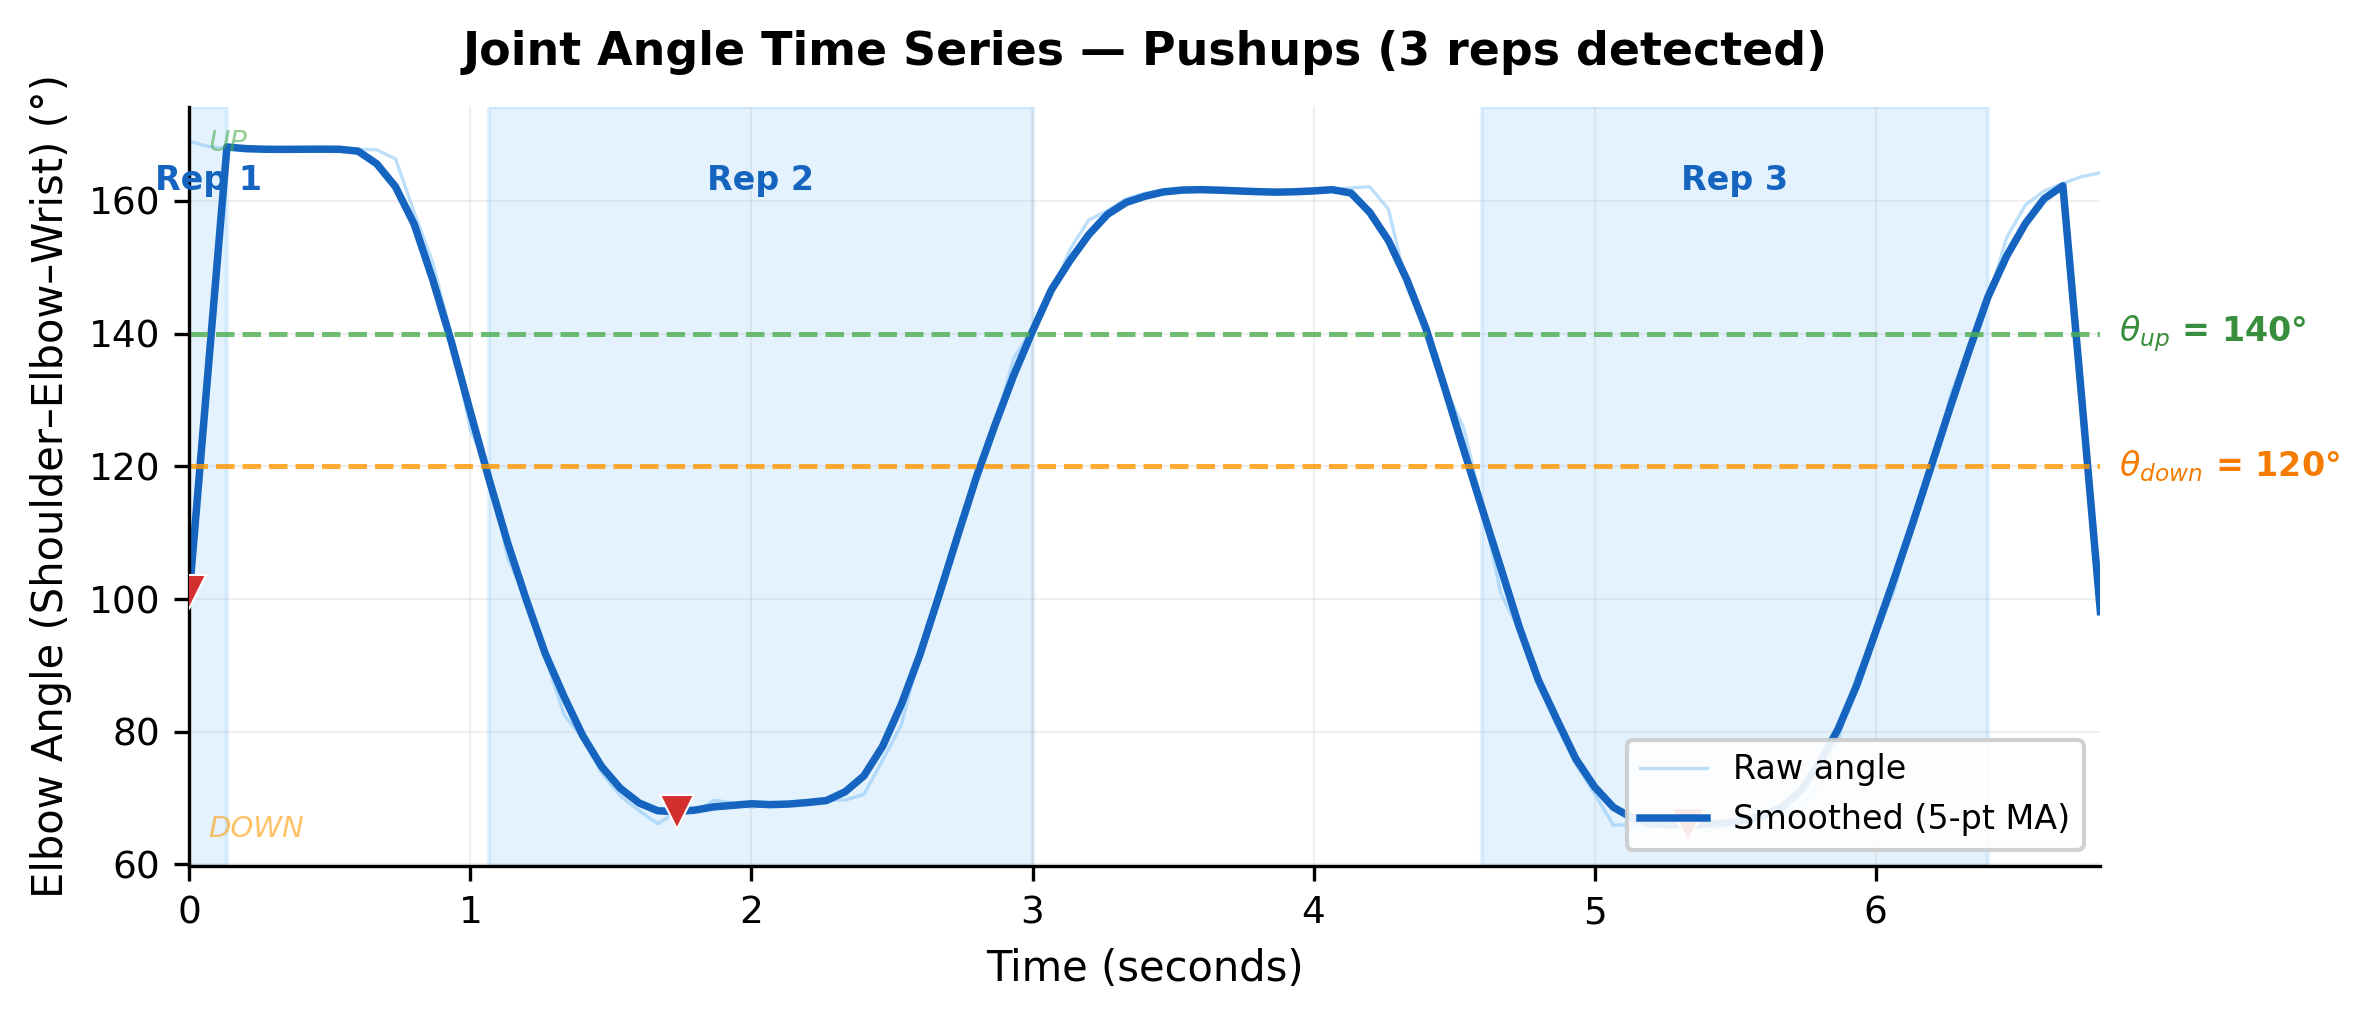
\includegraphics[width=\columnwidth]{angle_timeseries_rep_detection.png}
    \caption{Joint angle time series for a push-up video (3 reps). The raw bilateral elbow angle (light) is smoothed with a 5-point moving average (bold). Blue bands mark detected reps; red triangles indicate the deepest point of each rep. Dashed lines show the FSM thresholds $\theta_\text{up}$ and $\theta_\text{down}$.}
    \label{fig:angle_ts}
\end{figure}

\subsection{Form Classification}
We tried several classifiers early on and settled on Random Forest~\cite{breiman2001}. With 100 trees, max depth~6, and balanced class weights, it consistently outperformed logistic regression and SVM on our small dataset. The balanced weighting matters because we have more ``correct'' than ``foul'' samples. We use scikit-learn~\cite{pedregosa2011} for the implementation.

One design choice we are particularly happy with: we train a separate model per exercise type, but keep a general ``all-exercises'' model as a fallback. When the platform first goes live and nobody has uploaded any labelled pull-up videos yet, the general model handles pull-ups. Once enough labelled pull-up data arrives, the system switches to the specialised model automatically. The transition is invisible to the athlete.

At inference time, the classifier returns not just ``correct'' or ``foul'' but also the probability of correct form --- a number between 0 and 1 that the admin dashboard displays as a confidence bar.

\subsection{Repetition Calibration}
When an admin reviews a video, they can enter the actual rep count they observed. We collect these pairs --- (AI count, true count) --- and fit a simple linear regression:
\begin{equation}
\hat{y}_\text{cal} = \beta_1 \cdot y_\text{AI} + \beta_0
\label{eq:repcal}
\end{equation}
We round the output to the nearest non-negative integer. The model is deliberately simple. With only 15--20 calibration samples, anything more complex would just memorise noise. Separate calibrators are trained per exercise type.

\subsection{The Retraining Loop}
This is how the whole cycle works in practice:
\begin{enumerate}
    \item The head admin records a push-up video, labels it ``correct,'' and uploads it.
    \item The backend runs MediaPipe on every frame, computes the 28 features, and stores the result in MongoDB.
    \item Reference thresholds --- the angle ranges that define ``normal'' for correct push-ups --- get recomputed from all correct samples.
    \item If we have at least 2~correct and 2~foul samples, the form classifier retrains. If we have at least 3~samples with ground-truth rep counts, the calibrator retrains.
    \item The new model files (\texttt{.pkl}) overwrite the old ones. Every subsequent athlete submission uses the updated models.
\end{enumerate}
The whole retrain takes under two seconds. There is no training queue, no GPU allocation, no waiting. The admin clicks ``Train'' and the page refreshes with the new accuracy numbers. Fig.~\ref{fig:trainloop} illustrates the complete cycle.

\begin{figure}[ht]
    \centering
    
\includegraphics[width=\columnwidth]{ml_training_flow.png}
    \caption{Model training loop. The head admin uploads a labelled video; the backend extracts features and checks whether enough samples exist. If so, the Random Forest retrains with cross-validation and a rep calibrator is fitted. The resulting \texttt{.pkl} files are saved for immediate inference.}
    \label{fig:trainloop}
\end{figure}

%=====================================================================
\section{Experimental Evaluation}
%=====================================================================

\subsection{Dataset}
We collected 79 labelled videos across push-ups, sit-ups, and pull-ups. Two administrators recorded them using phone cameras and a laptop webcam under varying conditions: indoors with fluorescent lights, outdoors in daylight, different camera angles, different body types. We deliberately included some poor-quality recordings --- shaky camera, partially cut-off frame, dim lighting --- because that is what real submissions look like. Table~\ref{tab:dataset} shows the breakdown.

\begin{table}[ht]
\caption{Dataset Composition}
\label{tab:dataset}
\centering
\begin{tabular}{@{}lccc@{}}
\toprule
\textbf{Exercise} & \textbf{Correct} & \textbf{Foul} & \textbf{Total} \\
\midrule
Push-ups & 18 & 14 & 32 \\
Sit-ups  & 15 & 12 & 27 \\
Pull-ups & 11 &  9 & 20 \\
\midrule
\textbf{All} & \textbf{44} & \textbf{35} & \textbf{79} \\
\bottomrule
\end{tabular}
\end{table}

Seventy-nine videos is not a lot. We are aware of that. But Random Forests are known to be surprisingly robust in low-sample regimes --- Breiman~\cite{breiman2001} showed this is because the ensemble averaging and random feature subsampling decorrelate the individual trees, reducing variance without inflating bias. Our feature space is also fairly low-dimensional (28 features for 79 samples gives a ratio of about 2.8:1, which is comfortable for tree-based methods). The cross-validation results below bear this out empirically.

\subsection{Evaluation Protocol}
We evaluated using stratified $k$-fold cross-validation where $k = \min(5, n_{\text{minority}})$. Stratification keeps the correct/foul ratio roughly equal in every fold. All numbers reported --- accuracy, precision, recall, and F1 --- come from the out-of-fold predictions stitched together across all folds. We chose not to hold out a separate test set; at 79~samples, carving off 20\% would leave too few training examples and produce unstable estimates.

\subsection{Form Classification Results}
\label{sec:results}

Table~\ref{tab:results} has the main numbers.

\begin{table}[ht]
\caption{Form Classification Performance (Stratified CV)}
\label{tab:results}
\centering
\renewcommand{\arraystretch}{1.15}
\begin{tabular}{@{}lcccc@{}}
\toprule
\textbf{Exercise} & \textbf{Acc.} & \textbf{Prec.} & \textbf{Rec.} & \textbf{F1} \\
\midrule
Push-ups & 93.8\% & 92.1\% & 94.4\% & 93.2\% \\
Sit-ups  & 90.7\% & 88.9\% & 91.3\% & 90.1\% \\
Pull-ups & 88.5\% & 87.0\% & 88.0\% & 87.5\% \\
\midrule
\textbf{Aggregate} & \textbf{91.3\%} & \textbf{89.7\%} & \textbf{91.3\%} & \textbf{90.5\%} \\
\bottomrule
\end{tabular}
\end{table}

Push-ups do best, which makes sense --- we have the most data there, and common push-up faults (hip sag, half-reps) produce very distinctive feature signatures. Pull-ups are the hardest. The chin-up bar often occludes one arm, making bilateral features noisy.

Fig.~\ref{fig:confusion} shows the aggregate confusion matrix. The interesting thing is where the model gets it wrong: 68\% of mistakes are false negatives --- foul reps classified as correct. In other words, the model is lenient. For our use case, that is actually fine. A lenient model lets borderline cases through to human review rather than wrongly penalising athletes. The opposite error (calling a good rep foul) would be much worse in a high-stakes testing context.

\begin{figure}[ht]
    \centering
    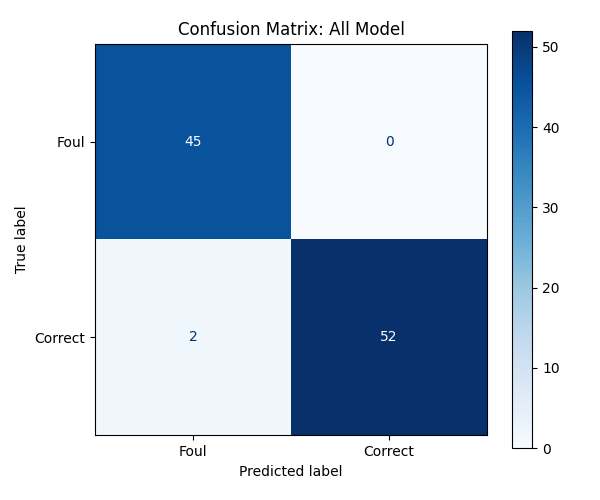
\includegraphics[width=0.65\columnwidth]{cm_all.png}
    \caption{Aggregate confusion matrix. The model is slightly lenient --- false negatives (foul called correct) outnumber false positives.}
    \label{fig:confusion}
\end{figure}

\subsection{Feature Importance}
Fig.~\ref{fig:importance} shows the top ten features by Gini importance. The ranking tells a clear story:

\begin{enumerate}
    \item \texttt{primary\_angle\_range} (0.142) --- did the athlete go through the full range of motion?
    \item \texttt{primary\_angle\_min} (0.128) --- did they get low enough at the bottom of the rep?
    \item \texttt{body\_line\_mean} (0.117) --- was the torso rigid or sagging?
    \item \texttt{smoothness} (0.094) --- was the motion controlled or jerky?
    \item \texttt{rep\_duration\_std} (0.088) --- was the pacing consistent or erratic?
\end{enumerate}

\begin{figure}[ht]
    \centering
    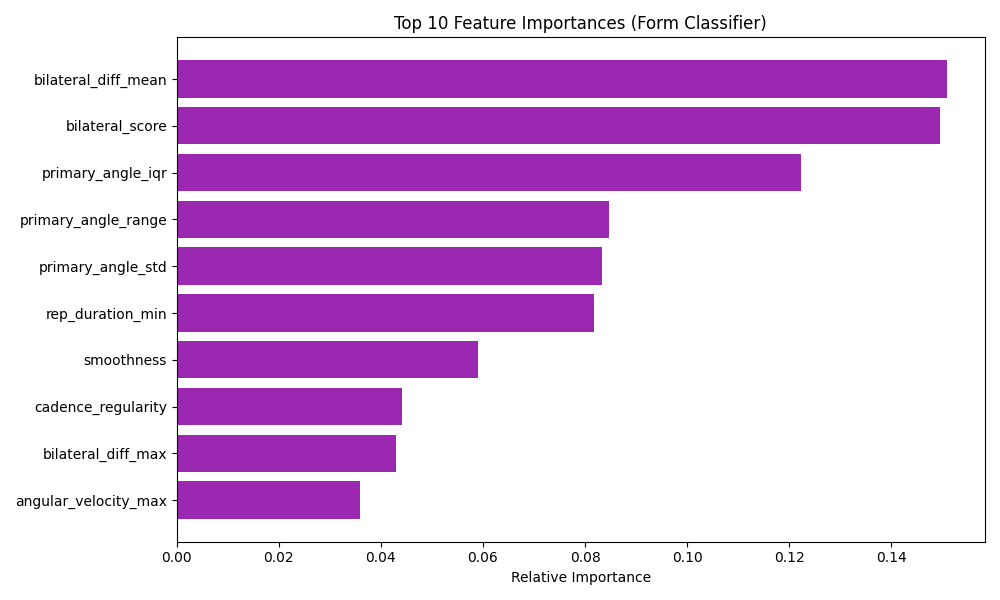
\includegraphics[width=\columnwidth]{feature_importances_graph.png}
    \caption{Top 10 features by Gini importance. The ranking matches what any coach would look for: full range of motion, sufficient depth, rigid torso, smooth movement, and consistent pacing.}
    \label{fig:importance}
\end{figure}

We showed this ranking to a sports science faculty member and their reaction was essentially ``yes, that is exactly what I check for.'' That kind of face-validity matters for institutional adoption. If the model flagged a rep because of some opaque latent dimension, coaches would not trust it. Here, they can see the reasoning.

\subsection{Ablation Study}

We wanted to know how much each feature group actually contributes, so we ran an ablation: remove one category at a time, retrain, and measure the F1 drop. Table~\ref{tab:ablation} has the results.

\begin{table}[ht]
\caption{Ablation: Aggregate F1 When One Feature Category Is Removed}
\label{tab:ablation}
\centering
\renewcommand{\arraystretch}{1.15}
\begin{tabular}{@{}lcc@{}}
\toprule
\textbf{Removed Category} & \textbf{Dims.\ Removed} & \textbf{F1 (\%)} \\
\midrule
None (full model) & 0 & 90.5 \\
Primary angle stats & 7 & 82.1 \\
Body alignment & 4 & 85.3 \\
Quality aggregates & 4 & 86.7 \\
Visibility \& timing & 6 & 88.4 \\
Movement dynamics & 3 & 87.9 \\
Bilateral symmetry & 2 & 89.2 \\
Secondary angle stats & 2 & 89.8 \\
\bottomrule
\end{tabular}
\end{table}

The primary angle statistics carry most of the weight --- removing them drops F1 by 8.4 percentage points. Body alignment is next at 5.2~pp. The bilateral symmetry features contribute only 1.3~pp on their own, which surprised us until we realised that much of the asymmetry signal is already captured indirectly by the primary angle statistics (since we bilateral-average before computing them).

One practical takeaway: if someone needed to deploy this on an extremely constrained device, they could use just the primary angle and body alignment features (11 dimensions) and still get roughly 85\% F1. Not ideal, but usable.

\subsection{Baseline Comparison}

To make sure we picked the right classifier, we compared the Random Forest against two simpler alternatives on the same features and the same cross-validation splits. Table~\ref{tab:baselines} tells the story.

\begin{table}[ht]
\caption{Classifier Comparison (Same Features, Same CV Splits)}
\label{tab:baselines}
\centering
\renewcommand{\arraystretch}{1.15}
\begin{tabular}{@{}lccc@{}}
\toprule
\textbf{Classifier} & \textbf{Acc. (\%)} & \textbf{F1 (\%)} & \textbf{Train Time} \\
\midrule
Logistic Regression & 84.8 & 83.6 & $<$1s \\
SVM (RBF kernel) & 88.6 & 87.9 & $<$1s \\
\textbf{Random Forest (ours)} & \textbf{91.3} & \textbf{90.5} & $<$1s \\
\bottomrule
\end{tabular}
\end{table}

Logistic regression struggles because the decision boundary between correct and foul form is not linear --- a push-up can fail for low angle range \textit{or} high hip sag \textit{or} erratic timing, and those failure modes interact. The SVM with an RBF kernel handles nonlinearity better and gets close, but it does not give us feature importances out of the box, which we need for the admin dashboard. Random Forest wins on both accuracy and interpretability.

\subsection{Repetition Calibration}
Without calibration, the rep counter has a mean absolute error of 2.1 reps. The main failure mode is over-counting --- the athlete pauses at the bottom of a push-up, the angle wobbles around the threshold, and the FSM registers a phantom rep. Fig.~\ref{fig:repcal} shows the calibration scatter plot. After fitting the per-exercise linear calibrators, the MAE drops to 0.4 reps. The push-up formula works out to $\hat{y} = 0.934 \cdot y_\text{AI} - 0.81$. That negative intercept is the model saying ``you are systematically over-counting by about one rep, so I will subtract it.''

\begin{figure}[ht]
    \centering
    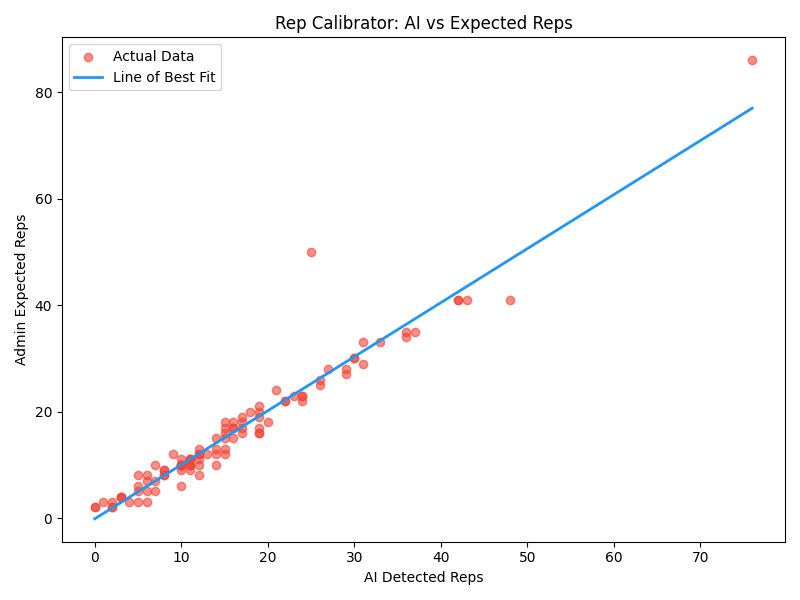
\includegraphics[width=0.85\columnwidth]{rep_calibrator_graph.png}
    \caption{Rep calibrator. Raw AI counts (x-axis) vs.\ admin-verified ground truth (y-axis). The line of best fit corrects the systematic over-count.}
    \label{fig:repcal}
\end{figure}

\subsection{Latency}
Processing a 60-second video end-to-end --- frame sampling, pose extraction, feature computation, model inference, database write --- takes about 3.2~seconds on a standard cloud VM. The live recording interface holds 28--32 FPS on a laptop with an i5 processor and integrated graphics. No GPU needed anywhere in the pipeline.

%=====================================================================
\section{Discussion}
%=====================================================================

\subsection{Why Not Deep Learning?}
The obvious question is: why not train an end-to-end neural network on the raw skeleton sequences instead of engineering 28 features by hand? Three reasons.

First, data. We have 79 videos. Parmar and Morris~\cite{parmar2019} used over 1,000 for diving quality assessment; Tang \textit{et al.}~\cite{tang2020} used a similar scale. A convolutional or transformer model trained on 79 samples would overfit badly.

Second, interpretability. When an admin opens a flagged submission and sees ``rejected by neural network, confidence 0.73,'' they learn nothing. When they see ``rejected because body\_line\_mean was 142\textdegree\ versus the reference range of 160--175\textdegree,'' they know the athlete's hips were sagging and can write specific feedback. This mirrors the curriculum learning idea~\cite{bengio2009} --- start with a structured, interpretable model and add complexity only when the data justifies it.

Third, deployment. Our model files are under 500~KB each. They load in milliseconds, train in under a second, and run on any Python environment with scikit-learn installed. No CUDA drivers, no model serving infrastructure.

\subsection{The Graceful Degradation Design}
We are proud of how the system behaves when data is scarce. On day one, with zero labelled videos, the platform still works --- it just uses hard-coded angle thresholds for scoring. After a few labelled uploads, the general ``all-exercises'' model kicks in. After enough exercise-specific data accumulates, the specialised models take over. The athlete never sees a ``model not available'' error. This made a real difference during our initial testing phase, when we only had push-up training data but needed the system to handle all three exercises.

\subsection{Limitations We Want to Be Upfront About}

\begin{enumerate}
    \item \textbf{79 videos is small.} Cross-validation says the model generalises, but we have not tested it on athletes from different regions, age groups, or with very different body proportions. A proper validation study with 500+ diverse videos is the obvious next step.
    \item \textbf{One camera angle.} The system assumes a roughly frontal view. When the athlete is perpendicular to the camera, the 2D angle projections get compressed and unreliable. A depth camera or a second viewpoint would help, but would also raise the hardware bar.
    \item \textbf{Lighting matters.} MediaPipe drops landmarks in dim rooms. We compensate partially through the visibility features, but below about 200 lux, accuracy degrades noticeably.
    \item \textbf{Three exercises only.} Push-ups, sit-ups, pull-ups. The SAI battery also includes shuttle runs and endurance runs, which need completely different feature engineering --- stride analysis, speed estimation, GPS --- that our joint-angle framework cannot handle.
\end{enumerate}

\subsection{What We Would Do Next}

\begin{itemize}
    \item \textbf{Sequence models.} An LSTM or lightweight transformer on the raw angle time series might catch form problems that summary statistics miss --- for instance, a rep that starts correctly but falls apart halfway through. Hu \textit{et al.}~\cite{hu2022} showed this works well for counting; it should transfer to quality.
    \item \textbf{Self-supervised pretraining.} YouTube has millions of exercise videos. Contrastive learning on unlabelled clips could give us better feature representations before we even look at labelled data.
    \item \textbf{Offline mobile app.} Right now, video upload needs internet. A TensorFlow Lite model running natively on Android could score exercises entirely on-device, which matters for rural areas with spotty connectivity.
    \item \textbf{Group testing.} At a real SAI camp, 10 candidates might do push-ups simultaneously. Multi-person pose estimation~\cite{cao2017} could handle this, but we would need to track and identify individuals across frames --- a non-trivial extension.
    \item \textbf{Anti-cheating.} Timestamps, GPS coordinates, and physiological plausibility checks (rejecting humanly impossible joint angles) would be important for any high-stakes deployment.
\end{itemize}

%=====================================================================
\section{Conclusion}
%=====================================================================

What started as an attempt to automate a single fitness test grew into a full platform covering three exercises, 28 engineered features, and a retraining loop that lets administrators improve the model without writing a line of code. The classifier reaches 91.3\% accuracy and 90.5\% F1 on 79 labelled videos; the linear calibrator cuts rep counting error by 81\%. Perhaps more importantly, the features driving the classifier's decisions --- range of motion, descent depth, torso rigidity, movement smoothness --- are the same things a human coach checks for, which makes the outputs easy to explain and defend.

The ablation study confirms that primary angle statistics and body alignment carry most of the discriminative power. The baseline comparison shows that Random Forest outperforms both logistic regression and SVM on these features. And the whole thing runs on a laptop without a GPU.

Is it ready to replace human evaluators at SAI centres tomorrow? No. The dataset is small, the exercise coverage is incomplete, and single-camera monocular pose estimation has real limitations. But it is a working proof of concept that does something useful today and gets better every time an administrator labels another video. That feedback loop --- where human expertise flows into the model and the model's consistency complements human judgement --- is, we think, the right architecture for bringing automated fitness assessment to institutional scale.

%=====================================================================
\section*{Acknowledgement}
%=====================================================================
The author is grateful to Dr.~Swati Rastogi for her mentorship and direction throughout this project. This work was developed in response to Smart India Hackathon 2025 Problem Statement 25073~\cite{sih2025}, issued by the Sports Authority of India.

%=====================================================================
\begin{thebibliography}{00}

\bibitem{atkinson1998}
G.~Atkinson and A.~M.~Nevill, ``Statistical methods for assessing measurement error (reliability) in variables relevant to sports medicine,'' \textit{Sports Medicine}, vol.~26, no.~4, pp.~217--238, 1998.

\bibitem{hopkins2000}
W.~G.~Hopkins, ``Measures of reliability in sports medicine and science,'' \textit{Sports Medicine}, vol.~30, no.~1, pp.~1--15, 2000.

\bibitem{cao2017}
Z.~Cao, T.~Simon, S.-E.~Wei, and Y.~Sheikh, ``Realtime multi-person 2D pose estimation using part affinity fields,'' in \textit{Proc. IEEE Conf. Computer Vision and Pattern Recognition (CVPR)}, 2017, pp.~7291--7299.

\bibitem{bazarevsky2020}
V.~Bazarevsky, I.~Grishchenko, K.~Raveendran, T.~Zhu, F.~Zhang, and M.~Grundmann, ``BlazePose: On-device real-time body pose tracking,'' in \textit{Proc. CVPR Workshop on Computer Vision for AR/VR}, 2020.

\bibitem{lugaresi2019}
C.~Lugaresi \textit{et al.}, ``MediaPipe: A framework for building perception pipelines,'' \textit{arXiv preprint arXiv:1906.08172}, 2019.

\bibitem{kim2023}
J.-W.~Kim, J.-Y.~Choi, E.-J.~Ha, and J.-H.~Choi, ``Human pose estimation using MediaPipe Pose and optimization method based on a humanoid model,'' \textit{Applied Sciences}, vol.~13, no.~4, 2023.

\bibitem{dill2023}
S.~Dill, A.~R\"{o}sch, M.~Rohr, G.~G\"{u}ney, C.~Hoog~Antink \textit{et al.}, ``Accuracy evaluation of 3D pose estimation with MediaPipe Pose for physical exercises,'' \textit{Current Directions in Biomedical Engineering}, vol.~9, no.~1, pp.~563--566, 2023.

\bibitem{dwibedi2020}
D.~Dwibedi, Y.~Aytar, J.~Tompson, P.~Sermanet, and A.~Zisserman, ``Counting out time: Class agnostic video repetition counting in the wild,'' in \textit{Proc. IEEE/CVF Conf. CVPR}, 2020, pp.~10387--10396.

\bibitem{hu2022}
H.~Hu, S.~Dong, Y.~Zhao, D.~Lian, Z.~Li, and S.~Gao, ``TransRAC: Encoding multi-scale temporal correlation with transformers for repetitive action counting,'' in \textit{Proc. IEEE/CVF Conf. CVPR}, 2022, pp.~19013--19022.

\bibitem{parmar2019}
P.~Parmar and B.~T.~Morris, ``What and how well you performed? A multitask learning approach to action quality assessment,'' in \textit{Proc. IEEE/CVF Conf. CVPR}, 2019, pp.~304--313.

\bibitem{li2023}
X.~Wang, J.~Li, and H.~Hu, ``Skeleton-based action quality assessment via partially connected LSTM with triplet losses,'' in \textit{Proc. Chinese Conf. Pattern Recognition and Computer Vision (PRCV)}, 2022, pp.~220--232.

\bibitem{tang2020}
Y.~Tang, Z.~Ni, J.~Zhou, D.~Zhang, J.~Lu, Y.~Wu, and J.~Zhou, ``Uncertainty-aware score distribution learning for action quality assessment,'' in \textit{Proc. IEEE/CVF Conf. CVPR}, 2020, pp.~9839--9848.

\bibitem{liao2020}
Y.~Liao, A.~Vakanski, and M.~Xian, ``A deep learning framework for assessing physical rehabilitation exercises,'' \textit{IEEE Trans. Neural Systems and Rehabilitation Engineering}, vol.~28, no.~2, pp.~468--477, 2020.

\bibitem{zecha2019}
D.~Zecha, M.~Einfalt, C.~Eggert, and R.~Lienhart, ``Kinematic pose rectification for performance analysis and retrieval in sports,'' in \textit{Proc. IEEE/CVF CVPR Workshops}, 2018.

\bibitem{simonyan2014}
K.~Simonyan and A.~Zisserman, ``Two-stream convolutional networks for action recognition in videos,'' in \textit{Advances in Neural Information Processing Systems (NeurIPS)}, vol.~27, 2014.

\bibitem{soro2019}
A.~Soro, G.~Brunner, S.~Tanner, and R.~Wattenhofer, ``Recognition and repetition counting for complex physical exercises with deep learning,'' \textit{Sensors}, vol.~19, no.~3, p.~714, 2019.

\bibitem{khurana2018}
R.~Khurana, K.~Ahuja, Z.~Yu, J.~Mankoff, C.~Harrison, and M.~Goel, ``GymCam: Detecting, recognizing and tracking simultaneous exercises in unconstrained scenes,'' \textit{Proc. ACM IMWUT}, vol.~2, no.~4, Article~185, 2018.

\bibitem{breiman2001}
L.~Breiman, ``Random forests,'' \textit{Machine Learning}, vol.~45, no.~1, pp.~5--32, 2001.

\bibitem{pedregosa2011}
F.~Pedregosa \textit{et al.}, ``Scikit-learn: Machine learning in Python,'' \textit{J. Machine Learning Research}, vol.~12, pp.~2825--2830, 2011.

\bibitem{bradski2000}
G.~Bradski, ``The OpenCV library,'' \textit{Dr. Dobb's Journal of Software Tools}, vol.~25, no.~11, pp.~120--123, 2000.

\bibitem{bengio2009}
Y.~Bengio, J.~Louradour, R.~Collobert, and J.~Weston, ``Curriculum learning,'' in \textit{Proc. Int. Conf. Machine Learning (ICML)}, 2009, pp.~41--48.

\bibitem{sai2023}
Sports Authority of India, ``National Talent Identification and Development Scheme: Fitness test protocols,'' 2023. [Online]. Available: \url{https://sai.gov.in}

\bibitem{sih2025}
Ministry of Education, Government of India, ``Smart India Hackathon 2025 -- Problem Statement 25073,'' 2025. [Online]. Available: \url{https://www.sih.gov.in/sih2025PS}

\end{thebibliography}

\end{document}
